\chapter{Introduction}\label{grammar-intro}

\section{Aims of this grammar}

This work is the first comprehensive description of the Yakkha language  (\textsc{iso}-639: ybh), a Kiranti language spoken in Eastern \isi{Nepal}. The primary focus of this work is on the dialect spoken in Tumok village. 

The grammar is intended to serve as a reference to scholars interested in linguistic typology and comparative studies of \isi{Tibeto-Burman} and Himalayan languages in general, and also as a foundation for members of the Yakkha community to aid future research and activities aiming at documenting and preserving their language. 

The grammar is written in a typological framework.  Wherever possible I have tried to incorporate a historical perspective and comparative data in explaining how a particular subsystem of the grammar works. For the sake of reader friendliness and to ensure long-term comprehensibility, the analyses are not presented within any particular theoretical framework, and terms that strongly imply a particular theory have been avoided as far as this was possible.  

Preparing a grammar can be a simultaneously  satisfying and frustrating task, both for the same reason: the sheer abundance of topics one has to deal with, which makes grammars very different from works that pursue more specific questions. Necessarily, a focus had to be set for this work, which eventually fell on morphosyntactic issues. Verbal inflection, \isi{transitivity}, grammatical relations, nominalization, complex predication and clause linkage are dealt with in greater detail, while other topics such as phonology, the \isi{tense}/\isi{aspect} system and \isi{information structure} leave much potential for further research. Since this is the first grammatical description of Yakkha, I have decided to include also the topics that are analyzed in less detail, in order to share as much as possible about this complex and intriguing language.


\section{How to use the grammar}\label{how-to}

\subsection{Structure of the book}


Following the well-established traditional order, I will provide some background on the langauge and its speakers (Chapter \ref{languageintro}), and treat the most important grammatical aspects of the language successively: phonology (Chapter \ref{phon}), morphology (Chapters \ref{ch-pron} – \ref{verb-verb}), syntax (Chapters \ref{verb-val} – \ref{clink-rest}) and, albeit briefly, discourse-structural particles and \isi{interjections} (Chapter \ref{particles}). \sectref{overview-yakkha} in this chapter provides a typological overview and highlights the main features of Yakkha by means of simple examples. Appendices contain (a) three narrative texts and  (b) charts with the complex \isi{kinship} terminology. The book also includes  a subject index and an index to the grammatical morphemes found in Yakkha, in order to make the information on particular topics easily accessible. 
\todo{We need to \textbackslash define chapref - Warum? Sieht doch alles gut aus.}

\subsection{Orthography and transliterations}\label{orth}

The \isi{orthography} used in this grammatical description does not represent the phonetic level, because it is impractical to note down every phonetic difference and individual variation, especially since a phonetic analysis is not the major goal of this work. The \isi{orthography} does not represent the phonemic level either, because Yakkha has a complex system of morphophonological rules, so that the pronunciation may show considerable deviations from the underlying forms. This is the reason why I use a representation on the allophonic level, including allophones that are the result of \isi{voicing}, assimilations and other morphophonological operations. Most examples in Chapter \ref{phon} on the phonology  are supplemented by the underlying forms (in slashes), in order to demonstrate the morphophonological processes.

While the  \isi{orthography} employed here is based on \textsc{ipa}, some deviations have to be noted: following the common orthographic traditions found in descriptions of \isi{Tibeto-Burman} languages, the symbol <y> is used for the palatal approximant (\textsc{ipa}: [j]), <c> is used for the alveolar fricative (\textsc{ipa}: [ts]), and <ch> stands for its aspirated counterpart (\textsc{ipa}: [tsʰ]). Aspirated consonants are written <ph>, <th>, <kh>, <wh>, <mh>, <nh>, <ŋh>. Geminated consonants are written with double letters, e.g., [mm] or [ss]. Yakkha has several prefixes that have the phonemic value of an unspecified  nasal. The nasal assimilates to the place of articulation of the following consonant. I do not use a special character for the nasal, but write it as it appears, i.e., as [m], [n] or [ŋ]. If the underlying form is provided, it is written /N/. 

\ili{Nepali} lexemes, used for instance when referring to sources of loans, are provided in the International Alphabet of Sanskrit Transliteration (\textsc{iast}). Common place names are generally not transliterated, but provided in a simplified \isi{orthography} that is generally found in local maps.

Yakkha does not have a writing tradition, but over the last few decades a few written materials have been published locally (cf. \sectref{earlier-work}), using the \isi{Devanagari} script, with varying orthographies. \isi{Devanagari} is not ideal for Yakkha because it does not have a grapheme for the glottal stop, but a number of solutions have been used in these language materials, such as writing <ʔ>  or using the grapheme for a central vowel <{\Deva अ}> together with a \emph{virām} <{\Deva  ्}>  (indicating that the inherent vowel should not be pronounced in the \isi{Devanagari} script).  \isi{Devanagari} is not used in this book, but  I have used the option that incorporates <ʔ> into \isi{Devanagari} in the \isi{Yakkha-Nepali-English dictionary} that has been composed alongside this grammar.\footnote{Cf. http://dianaschackow.de/?nav=dictionary.}


\subsection{Glossing and further conventions}

The purpose of the glosses is to facilitate understanding the examples, which necessarily entails a simplification of the facts. The labels used in the glosses do not represent analyses. This is particularly important with regard to the person inflection. As is typical for Kiranti languages, an inflected form cannot be neatly segmented into straightforward form-function correspondences (though from a  Kiranti perspective, the verbal inflection of Yakkha can be considered as rather simple). To provide an example, the transitive \isi{person marking} on the verbs has labels such as \rede{1pl.A} (for the marker \emph{-m}) in the glosses, so that the reader can identify the reference of a marker in a particular person configuration. The actual distribution of these markers is likely to be more narrow or wider than the gloss labels suggest (cf. \sectref{verb-infl}). But glossing the above-mentioned marker with \rede{1/2pl.A>3.P}, for instance, would result in cryptic glosses that make reading the examples a rather cumbersome task. 

Categories that have no corresponding overt marker, such as the subjunctive, are represented in square brackets, e.g., [{\sc sbjv}]. This may have two reasons: either the morpheme is zero, or the morpheme got deleted in the surface form due to morphophonological processes. The \isi{nominative}, which is also zero, is never written in the glosses. It is implied when a noun appears without an overt \isi{case} marker. 

The category labels are congruent with the Leipzig Glossing Rules,\footnote{Cf. http://www.eva.mpg.de/lingua/resources/glossing-rules.php.} with Yakkha-specific category labels added where necessary. All abbreviations are listed on page \pageref{abbreviations}. Language-specific morphological categories such as the Past Subjunctive \isi{mood} or the Ablative \isi{case} are capitalized, to distinguish them from universal categories.

When \isi{kinship} terms are used in the glosses, they are abbreviated according to common practice: lower \isi{case}  \emph{e} and \emph{y} stand for \rede{elder} and \rede{younger}, upper \isi{case} \emph{M} stands for \rede{mother}, \emph{F} stands for \rede{father}, \emph{Z} stands for \rede{sister}, \emph{B} stands for \rede{brother}, \emph{W} stands for \rede{wife}, \emph{H} stands for \rede{husband}, \emph{S} stands for \rede{son}, \emph{D} stands for \rede{daughter}. Combinations of them are read like possessive phrases, e.g., \emph{FeZH} stands for \rede{father's elder sister's husband}. 


In the texts, and in some of the \ili{Nepali} literature cited, the Bikram Sambat (also Vikram Samvat) calendar is used. This is the official calendar in \isi{Nepal}, and it is  56.7 years ahead of the solar Gregorian calendar. Sources using this system have \rede{B.S.} written behind the year.

The Yakkha examples that are provided in this grammar contain references to the corpus, in square brackets. Examples without such references are from elicitations that have not been recorded.


\subsection{Notes on terminology}\label{terminology}

\subsubsection{Nominalization}

Nominalization is a versatile strategy in Sino-Tibetan languages, and its functions reach well beyond the classical uses of nominalization, which has given rise to the term \emph{Standard Sino-Tibetan Nominalization} \citep{Bickel1999Nominalization}. Since also relative clauses, complement clauses and main clauses can be noun phrases structurally, the reader should note that this work employs a very liberal understanding of the term nominalization, as is commonly found in works on Sino-Tibetan languages. Alternatively, one could have made up new labels for each function of  a \isi{nominalizer}, such as \emph{attributivizer}, \emph{complementizer}, \emph{factuality marker}, but then, the functional connection between these uses would have been obscured, especially since grammars are rarely read chronologically. I found that this use of the term puzzled readers and hearers who are not familiar with Sino-Tibetan languages. Still, I decided to retain the label \emph{nominalization} in this work also for the less canonical uses of nominalization, in order to keep functional and historical connections maximally transparent.

A similar issue is the employment of \isi{case} markers in \isi{clause linkage}. I retained the \isi{case} labels also when these markers attach to (not necessarily nominalized) clauses as clause linkage markers. Especially if one \isi{case} marker is highly multifunctional in clause linkage, it is futile to find new labels for each function (the \isi{comitative} marker \emph{=nuŋ} is an example, see Chapter \ref{com-cl}).


\subsubsection{Generalized Semantic Roles (\textsc{gsr}s)}

I have analyzed Yakkha \isi{argument structure} and grammatical relations by looking at how generalized semantic roles (\textsc{gsr}) are realized and aligned in morphology and syntax, following the methodology of \citet{Bickel2010_Grammatical} and \citet{Witzlack2010_Typological}. \textsc{gsr}s are defined by their semantic properties and they are always determined in relation to a particular predicate. For instance, the most agent-like argument (A) of \emph{mokma} \rede{hit} is the hitter, and the most patient-like argument (P) is the hittee. The sole argument of an intransitive verb is the S argument. Analogously, one can identify the most goal-like argument (G) and the most theme-like argument (T) of three-argument constructions. The identification of \textsc{gsr}s purely follows semantics, and is determined regardless of how the arguments  are realized in morphology and syntax. For instance, the most agent-like arguments of \isi{experiential predicates} such as \rede{love} and \rede{be disgusted} (i.e., the experiencers) are realized as possessors in one particular verb class in Yakkha.  

Such an approach is necessary because Yakkha does not have a dominant \isi{alignment} type, and thus, a morphologically and syntactically consistent notion of subject and object cannot be determined. In converbal constructions, S and A align, while in \isi{case} marking and in some complement constructions S and P align. Nominalization and \isi{relativization} constructions present a mixed picture. Marginally (only in verbal \isi{person marking} and in complement clauses), the  privileged argument can also be determined by reference and by \isi{information structure}. The most bewildering diversity of \isi{alignment} types is found in the verbal \isi{person marking}.\footnote{This diversity is not random and has parallels in the related languages, cf. \sectref{verb-infl}.}   


The Yakkha verb, if transitive, shows agreement with both arguments. To identify the respective morphology, I use the terms \emph{(transitive) subject agreement}  and \emph{(transitive) object agreement}. It should be kept in mind that these labels do not imply any particular formally unified behavior, neither with respect to \isi{case} and \isi{person marking} nor with respect to the choice of pivots in any construction. In the glosses,  the labels A and P are used, since in the standard frame of \isi{argument realization} markers referred to by A index A arguments and markers referred to by P index P arguments. This need not be the case, however, as some \isi{experiencer} arguments might be realized as P morphologically, e.g., in experiential verbs such as \emph{khikma} \rede{taste bitter to someone} (cf. Chapter \ref{verb-val}).


\section{Data sources}\label{sources}

\subsection{Fieldwork}

The material used to write this grammar was collected during four field trips between 2009 and 2012, amounting to roughly one year altogether. I have spent most of the time in Tumok (\ili{Nepali}: Tamaphok) village, with occasional visits to the surrounding villages Waleng (\ili{Nepali}: Madi Mulkharka), Mamling, Yaiten (\ili{Nepali}:  Dandagaun), Hombong and to the market town Mudhe Saniscare. Tumok is a night's and half a day's bus ride away from Kathmandu (via Dharan, Dhankuta and Hile). One gets off the bus in  Mudhe Sanischare and walks down to Tumok village for another hour or two.\footnote{Alternatively, one may take a domestic flight to Tumlingtar and try to catch a bus or a jeep there, but since the transport situation was not reliable in Tumlingtar in 2009 and 2010, I resorted to making the journey to the east by bus in my later field trips (2011 and 2012).}


During the first field trip in 2009 Kamala Koyongwa travelled with me, helping me in many ways. From the first year on I stayed with Kamala Linkha, a teacher at the Shree Chamunde Higher Secondary School in Tumok, who became my friend and also my main Yakkha teacher, simply by sharing her everyday life with me. She  never grew tired of explaining her language and aspects of Yakkha life to me.  Magman Linkha, a teacher at the same school, has provided me with numerous beautifully-told narratives. He also  helped me to check transcriptions and dictionary entries, patiently answering my many questions. Since he is himself engaged in various activities aiming at documenting and preserving his cultural heritage, he was also my most important source regarding socio\-linguistic and ethnographic questions. In 2010, Kamala's niece Man Maya Jimi, a student who also works in adult literacy education programs, started working with me and proved to be a patient and thoughtful consultant in elicitations, transcriptions, translations and dictionary checks. In Kathmandu, I also had several valuable elicitation sessions with Kaushila Jimi and her son Sonam as well as with Visvakaji Kongren.


 \begin{figure}
 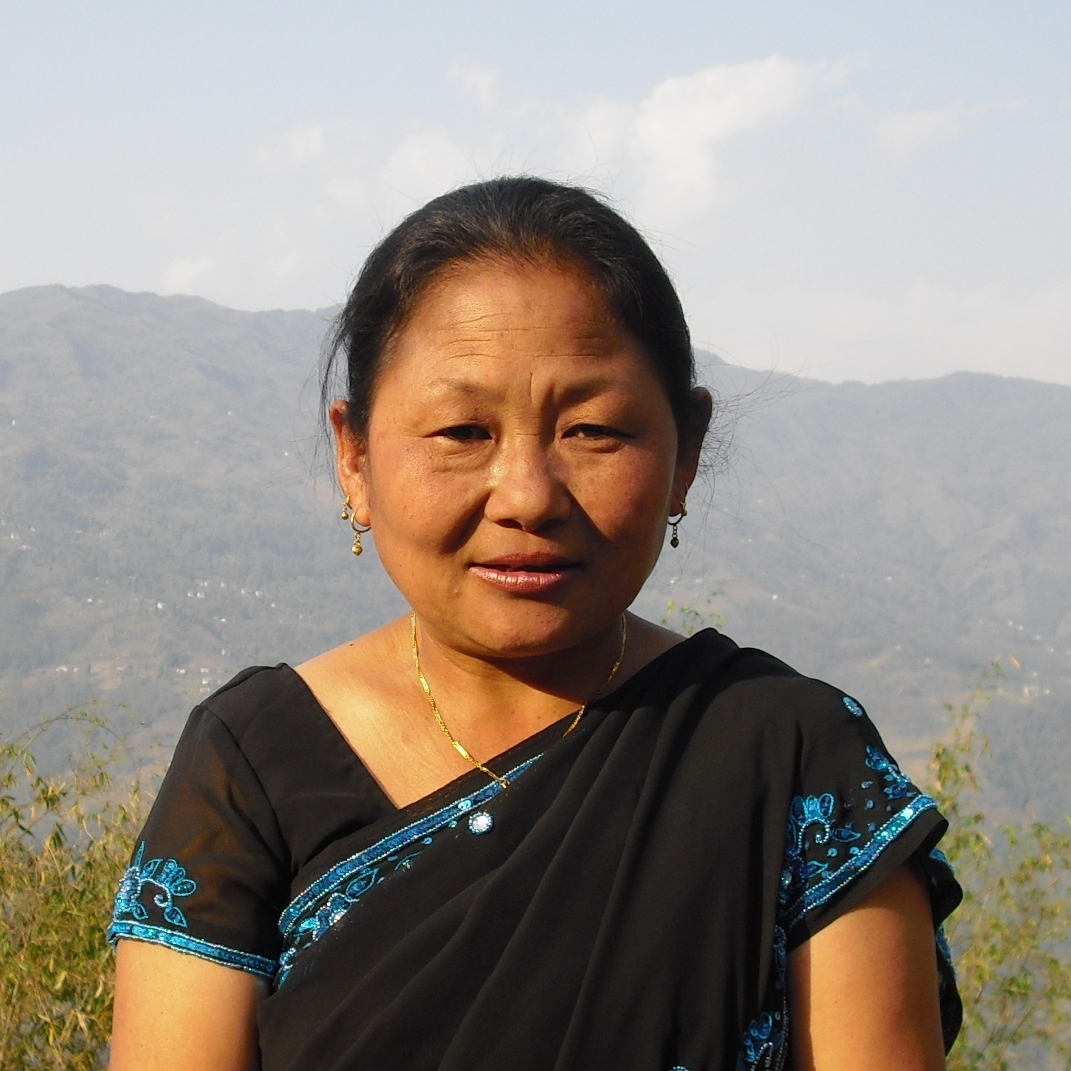
\includegraphics[width=0.30\textwidth]{figures/kamala.jpg}
 \hfill
 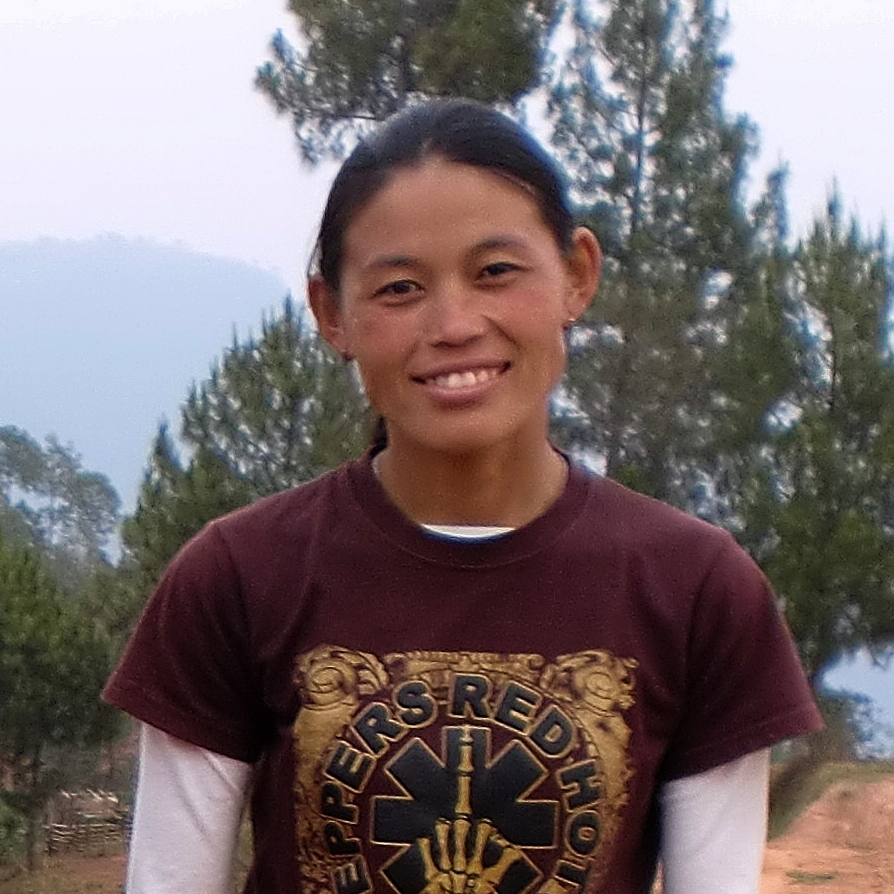
\includegraphics[width=0.30\textwidth]{figures/manmaya.jpg}
 \hfill
 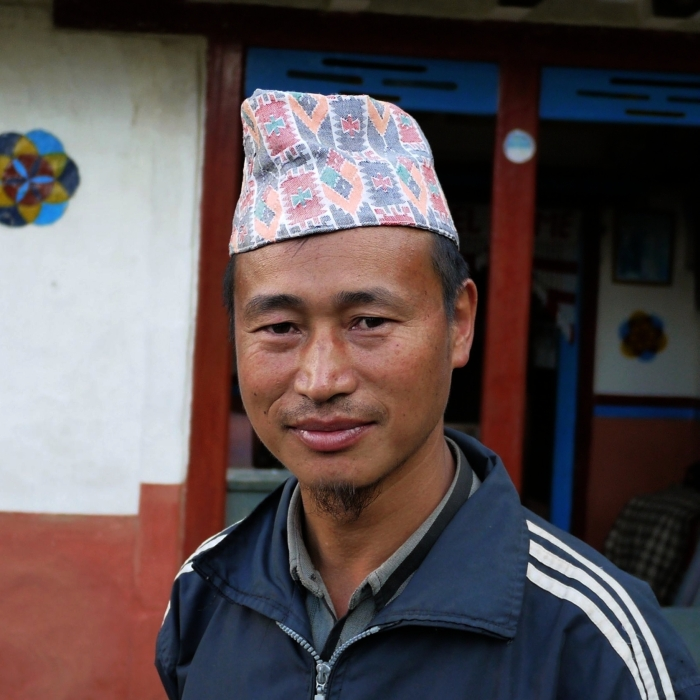
\includegraphics[width=0.30\textwidth]{figures/magman.jpg}
 \caption{My main Yakkha teachers: Kamala Linkha, Man Maya Jimi, Magman Linkha}
 \end{figure}

 
During the early trips (2009 and 2010) I recorded texts from various genres (legendary and autobiographical narratives, spontaneous conversations, songs, pear stories, procedural descriptions) and tried to gather as much language data as possible while living in the village. In total, I recorded utterances from 22 different speakers. The youngest person recorded was 16 years old, the oldest people were above 60 years. To each person recorded I have explained the purpose of the recordings and my plan to archive them online. Their consent is mostly found as part of the recordings, usually at the end of the files.  After analyzing the data in Germany, I used the later trips (2011 and 2012) mainly for refined elicitations and data checking, with the consultants mentioned above in Tumok and in Kathmandu. 

In the elicitations, relying on nonverbal stimuli in the natural environment proved to be much more productive than prepared questionnaires or audiovisual stimuli. The only stimuli that I have used were the Pear Story \citep{Chafe1980The-Pear} and the Cut and Break Clips \citep{Bohnemeyeretal2010_cut}. Questionnaires that were used included the questionnaire from the Leipzig Valency Classes Project (Max Planck Institute for Evolutionary Anthropology), the questionnaire from the project on referential hierarchies in three-participant constructions (University of Lancaster) and the Questionnaire for Transitivizing/Detransitivizing Verb Systems (by Johanna Nichols). The other topics were elicited with questionnaires compiled by myself and on the spot when certain topics came up during transcriptions and checks of the lexical data. Elicitations on clause linkage in 2012 were partly undertaken together with Lennart Bierkandt for a co-authored paper (\citealt{Bierkandtetal_Scope}).

\subsection{The corpus}\label{corpus}

The structure and content of the current Yakkha corpus is displayed in \tabref{tab-corpus}. The corpus contains 3012 clauses and roughly 13.000 annotated words. The texts are transcribed and annotated audio-recordings of roughly 3 hours length. The audio recorder used is an Olympus Linear \textsc{pcm} Recorder LS-11. The texts of the genre \emph{legacy data} are only available in written form, using \isi{Devanagari} script. They are taken from school books \citep{Jimi2009Engka-Yakkha, Jimi2010Engka-Yakkha} and from narratives that originated in a workshop organized in 2012 by the Mother Tongue Center \isi{Nepal} \citep{Jimee2012_Casuwa, Jimee2012_Owl, Linkha2012_Ashes}. I have transliterated them into the orthographic representation used in this work, with slight adjustments where the orthographies used  were rather impractical, for instance when they lumped together the voiceless and voiced consonants or /r/ and /l/ (which is the \isi{case} in the above-mentioned school books). Researchers using the corpus should be aware of the fact that many neologisms are used in written Yakkha that are not (yet) established in the spoken language. 




\begin{table}[htp]
\begin{center}
\begin{tabular}{lll}
\lsptoprule
{\sc genre}&{\sc \isi{number} of }&{\sc records}\\
& {\sc recordings}& (roughly corr. to clauses)\\
\midrule
narratives	&8&	488\\
conversations	&5&	1336\\
pear stories	&4	&225\\
songs	&3	&40\\
legacy data (written)	&5&	595\\
texts on tradition 	&3	&328\\
and material culture	&	&\\
\midrule
&28&\bf 3012\\
\lspbottomrule
\end{tabular}
\caption{Content of the annotated Yakkha corpus}\label{tab-corpus}
\end{center}
\end{table}


The texts are labelled as follows: a unique identifier, followed by an underscore and a three-letter genre code, followed by an underscore and the number of the text from that particular genre. For example, a text coded \rede{12\_nrr\_03.wav} is the twelfth recording in total and the third text of the genre \rede{narrative}; \rede{12\_nrr\_03.txt} is the corresponding text file. These labels (including the record number) are provided when the examples are from the corpus; when no such label is provided, the examples are from elicitations or from unrecorded spontaneous speech. The applications used for annotation and time \isi{alignment} were Toolbox\footnote{Toolbox is free software developed by \textsc{sil}, see http://www-01.sil.org/computIng/toolbox/index.htm.} and ELAN.\footnote{ELAN is free software developed by the Language Archive of the Max Planck Institute for Psycholinguistics in Nijmegen, see  \citet{Wittenburg2008_Annotation}; URL: http://tla.mpi.nl/tools/tla-tools/elan/;}

The genre codes are displayed in \tabref{tab-genre}.  The entire corpus is accessible online via the Endangered Languages Archive (\textsc{elar}).\footnote{http://www.hrelp.org/archive/. The annotations in this work may, in a few cases, deviate from the annotations in the archived corpus, as upon closer inspection during the analyses some minor adjustments were inevitable. The examples as they are analyzed and annotated in this work represent the most recent state of analysis.}

\begin{table}[htp]
\begin{center}
\begin{tabular}{ll}
\lsptoprule
{\sc code}&{\sc genre}\\
\midrule
nrr & narrative \\
cvs & conversation \\
sng & song\\
mat & description of material culture\\
tra & description of traditions\\
pea & pear story\\
par & elicited paradigm\\
leg & legacy data (written)\\
\lspbottomrule
\end{tabular}
\caption{Text genres and codes}\label{tab-genre}
\end{center}
\end{table}


\subsection{The lexical database}

The lexical database\footnote{Archived at the Endangered Languages Archive (\textsc{elar}) together with the corpus, see http://www.hrelp.org/archive/.} contains 2429 entries, all checked with at least two speakers. It contains grammatical, semantic, phonological and ethnographic notes as well as \isi{botanical terms} (relying on the \ili{Nepali} translations given in \citet{Manandhar2002_Plants} and occasionally \citealt{Turner1931A-Comparative}). One may also browse for parts of speech and for semantic categories, if one is interested in particular semantic domains like body parts, \isi{kinship}, spatial orientation, colour terms etc. A digital community version of the dictionary (using Lexique Pro),\footnote{See http://www.lexiquepro.com/.} with the Yakkha entries in \isi{Devanagari}, can be found online.\footnote{See http://dianaschackow.de/?nav=dictionary. Even though the database has been carefully checked, it is likely that further corrections and additions will be made in the future.}


\section{Earlier studies on Yakkha language and culture}\label{earlier-work}


Material on the Yakkha language that is available beyond local sources is exceedingly rare. The oldest source is a wordlist in \citet{Hodgson1857_Comparative}. A chapter in the Linguistic Survey of India provides a brief introduction and some Yakkha texts that were collected with Yakkha speakers who had migrated to Darjeeling \citep[305--315]{Grierson1909Linguistic}.\footnote{This source and \citet{Russell1992_Yakha} use a spelling <Yakha>, but the correct spelling is <Yakkha>, since the first \isi{syllable} is closed by /k/. In contemporary sources, also  in \isi{Devanagari}, the language name is always written as <Yakkha>.} 

More recent works on the language are a  glossary \citep{Winter1996Glossary}, a \isi{Yakkha-Nepali-English dictionary}  \citep{Kongren2007Yakkha}, two articles about the \isi{inflectional morphology}, both based on the same verbal paradigm collected by Gvozdanović \citep{Gvozdanovic1987How, Driem1994The-Yakkha} and an article by myself on three-argument constructions \citep{Schackow2012_Referential}.

Research on cultural and political aspects has been undertaken by \citet{Subba1999Politics} and by Russell \citep{Russell1992_Yakha, Russell1997Identity, Russell2000_Missing, Russell2004Traditions, Russell2007Writing, Russell2010_Perceptions}. Recently, two M.A. theses on aspects of Yakkha culture have been completed in \isi{Nepal}, one thesis on culture and adaptation by \citet{Rai2011_Nature}  and one thesis on \isi{kinship} terms by  \citet{Linkha2013_kinship}. Ethnographic introductions in \ili{Nepali} can be found by \citet{Kongren2007Indigenous} and by \citet{Linkha2067Yakkha}, the former containing also some English chapters. Further locally available materials in Yakkha and \ili{Nepali} are a collection of poems \citep{Dewan2001Opchyongme} and a  collection of thematically ordered wordlists and articles on the Yakkha traditions \citep{Linkha2005Yakkha}. For a more detailed bibliography of the works on Yakkha that were published in \ili{Nepali} the interested reader is referred to \cite{Rapachaetal2008Indo}. 

 

\section{Typological overview of the Yakkha language}\label{overview-yakkha}

The following brief overview is intended for the reader who is not familiar with Kiranti languages or other Sino-Tibetan languages in general. It provides basic information on the most important features of the language.

\subsection{Phonology}

Yakkha has five \isi{vowel phonemes} (/i/, /e/, /a/, /o/ and /u/). Diphthongs are rare and can mostly be traced back to disyllabic structures. The basic distinctions in the consonant phonemes, according to  the place of articulation, are bilabial, alveolar, retroflex, palatal, velar and glottal. Plosives, the affricate and the bilabial glide have an aspirated and an unaspirated series. The maximal \isi{syllable structure} is CCVC. Complex onsets originate in disyllabic structures too; they consist of sequences of obstruent and lateral, rhotic or glide. The \isi{syllable} coda is mainly restricted to \isi{nasals} and unaspirated plosives. The morphophonological processes are manifold and very complex in Yakkha, with each rule applying to its own domain (discussed in \sectref{morphophon}). A feature located at the boundary between phonology and morphology is a process of copying nasal morphemes in the verbal inflection (discussed in \sectref{sec-nasalcop}). This process is typical for Kiranti languages.


\subsection{Word classes}

Morphology and syntax clearly distinguish nominal and verbal classes in Yakkha (see Chapters \ref{ch-noun} and \ref{verbalmorph}). Word classes appearing in the \isi{noun phrase} are \isi{demonstratives}, pronouns,  \isi{quantifiers} and (marginally) \isi{numerals} (see Chapter \ref{ch-pron}). Numeral classification exists, but it plays only a very marginal role. The verb shows complex \isi{inflectional morphology}, resulting in hundreds of possibilities of inflection for each verbal stem. 


Less clear is the distinction of \isi{adjectives} and adverbs, as many of them derive from verbal roots. However, the salience of \isi{reduplication} and rhyming patterns in noun-modifying and verb-modifying lexemes justifies treating them as separate word classes (see Chapter \ref{adj-adv}). Rhyming and reduplications, often combined with ideophones, almost exclusively feature in the classes of \isi{adjectives} and adverbs in Yakkha.


Other word classes constitute closed classes, such as conjunctions, \isi{postpositions}, \isi{interjections} and discourse-structural particles (see Chapters  \ref{clink-rest} and \ref{particles}). The \isi{postpositions} are partly derived from \isi{relational nouns}. 


\subsection{Nominals}

Yakkha nouns can be simple or compounded out of several nominal roots. There are several nominalizers in Yakkha, some deriving nouns (\emph{-pa} and \emph{-ma}), some constructing noun phrases (\emph{-khuba, -khuma} and \emph{=na/=ha}).

 Nouns can be inflected by \isi{possessive prefixes}, alternatively to using \isi{possessive pronouns} (compare \Next[a] and \Next[b]). The \isi{possessive prefixes} are very similar in form to the \isi{possessive pronouns}. Case and \isi{number} markers are clitics; they attach to the whole \isi{noun phrase}. Yakkha has an unmarked \isi{nominative}, an \isi{ergative}/\isi{instrumental} \emph{=ŋa}, a \isi{genitive} \emph{=ka}, a \isi{locative} \emph{=pe}, an \isi{ablative} \emph{=phaŋ}, a \isi{comitative} \emph{=nuŋ}, and further markers with less central functions, mainly from the comparative domain. Argument marking shows reference-based and word class-based alternations (discussed in \sectref{nom-morph} for the \isi{ergative} \isi{case} and in \sectref{three-arg} for three-argument constructions).

\ex.\ag.a-paŋ=be\\ 
{\sc 1sg.poss-}house{\sc =loc}\\
\rede{in my house}
\bg.ak=ka paŋ=be\\
{\sc 1sg.poss=gen} house{\sc =loc}\\
\rede{in my house}


\subsection{Verbs}

The inflected verb  indexes agents and patients of transitive verbs and expresses many grammatical categories (\isi{tense}/\isi{aspect}, \isi{mood}, \isi{polarity} (see \Next). This example also shows the above-mentioned process of \isi{nasal copying}; suffix \emph{-m} appears twice in the suffix string. Person (including \isi{clusivity}), \isi{number} and \isi{syntactic role} marking interact in intricate ways in the \isi{person marking} paradigm (see \sectref{verb-infl}). As example \Next shows, the Yakkha verb is mainly suffixing; there is only one prefix slot. 

\exg.n-dund-wa-m-ci-m-ŋa-n=ha.\\
{\sc neg-}understand{\sc -npst-1pl.A-nsg.P-1sg.A-excl-neg=nmlz.nsg}\\
\rede{We do not understand them.}


Yakkha has a very productive system of complex predication, where several verbal roots are concatenated to yield a more specific verbal meaning (discussed in Chapter \ref{verb-verb}). In complex predicates, the first verb carries the lexical meaning, while the second verb adds a further semantic specificiation, for instance regarding aktionsart, the spatial directedness of the event, or the affectedness of some argument. In \Next, the second verb carries a \isi{benefactive} notion, adding a beneficiary argument to the \isi{argument structure} of the lexical verb. Complex predicates trigger \isi{recursive inflection}, as shown here by the \isi{imperative} marker \emph{-a}, that appears twice (treated in detail in Chapter \ref{verb-verb}). Predicates can also be compounded by a noun and a verb  (see Chapter \ref{noun-verb}).
 	
	\exg. ka katha lend-a-by-a-ŋ.\\
	{\sc 1sg} story  exchange{\sc -imp-V2.give-imp-1sg.P}\\
	\rede{Tell me a story.}



\subsection{Syntax}

Yakkha phrase structure is overwhelmingly  head-final, with the nominal head at the end of the \isi{noun phrase}, and with the verb being the final constituent of the clause (see \Next[a]). In complex clauses, the subordinate clause generally precedes the main clause (see \Next[b]). Nominalizers and markers of \isi{clause linkage} can follow the verb. Permutations of the word order are possible (see Chapter \ref{simp-cl}); they follow discourse requirements. Arguments are frequently dropped, resulting in a low referential density. 

\ex.\ag.raj=ŋa u-ma  kheps-u=na.\\
Raj{\sc =erg} {\sc 3sg.poss-}mother hear{\sc [pst]-3P=nmlz.sg}\\
\rede{Raj heard his mother.}
\bg.tumok=pe tas-u-ŋ=hoŋ a-phu chimd-u-ŋ=na.\\
Tumok{\sc =loc} arrive{\sc [pst]-3P-1sg.A=seq} {\sc 1sg.poss-}elder\_brother ask{\sc [pst]-3P-1sg.A=nmlz.sg}\\
\rede{When I arrived in Tumok,  I asked my elder brother (about it).}

The \isi{argument structure} in Yakkha distinguishes several \isi{valency} classes, discussed in Chapter \ref{verb-val}. The basic distinction is that between intransitive and transitive verbs, which is also reflected in two different verbal inflectional patterns. There is a class of \isi{labile verbs}, mostly showing an \emph{inchoative/causative} alternation. Experiential predicates predominantly occur in a construction that treats the \isi{experiencer} as the metaphorical possessor of a sensation or an affected body part (the Experiencer-as-Possessor Construction, see \Next).

\ex.\ag.a-pomma=ci ŋ-gy-a=ha=ci.\\
{\sc 1sg.poss-}laziness{\sc =nsg} {\sc 3pl-}come\_up{\sc -pst=nmlz.nsg=nsg}\\
\rede{I feel lazy.}
\bg.ka nda         a-luŋma  tuk-nen=na.\\
{\sc 1sg[erg]} {\sc 2sg} {\sc 1sg.poss-}liver pour{\sc -1>2[pst]=nmlz.sg}\\
\rede{I love you/I have compassion for you.}


The \isi{argument structure} can be modified, by means of derivations (causative), complex predication (\isi{benefactive}, middle, reflexive), and an analytical construction (reciprocal), as shown in \Next. Both the  reflexive and the  \isi{reciprocal construction} make use of a \isi{grammaticalization} of the verbal root \emph{ca}  \rede{eat}. 


\ex.\ag.kiba=ŋa hari kisi-met-u=na.\\
tiger{\sc =erg} Hari be\_afraid{\sc -caus-3.P[pst]=nmlz.sg}\\
\rede{The tiger frightened Hari.}
\bg. nda (aphai) moŋ-ca-me-ka=na.\\
\sc{2sg} (self) beat-\sc{V2.eat-npst-2=nmlz.sg}\\
\rede{You beat yourself.}
\bg. kanciŋ [...] sok-khusa ca-ya-ŋ-ci-ŋ.\\
\sc{1du}  [...] look-\sc{recip} eat\sc{.aux-pst-excl-du-excl}\\
\rede{We (dual, excl) looked at each other.}



Furthermore, morphologically unmarked detransitivizations are possible (marked only by a change in the \isi{person marking} morphology). In this way, both antipassive and passive constructions may occur in Yakkha, sometimes leading to ambiguities. In \Next, the person morphology on the verb is intransitive in both examples, signalling a third person singular subject of an intransitive verb, although \emph{khemma} \rede{hear} is clearly transitive, and in most cases is inflected transitively (compare with \Next[c]). While \Next[a] is a passive structure, \Next[b] is an antipassive. Unmarked antipassives (the morphosyntactic de\isi{motion} of a generic or unspecific object) are wide-spread in Kiranti languages, but unmarked passives are, to this point, only known in Yakkha. The more frequent structure is, however, the antipassive, which is not surprising given its older nature.

\ex.\ag. ceʔya kheps-a-m=ha.\\
matter hear{\sc [3sg]-pst-prf=nmlz.nc}\\
\rede{The matter has been heard.}
\bg. Dilu  reɖio khem-meʔ=na?\\
Dilu radio  hear{\sc [3sg]-npst=nmlz.sg}\\
\rede{Does Dilu listen to the radio (generally)?}
\bg. pik=ŋa kiba kheps-u=na.\\
cow{\sc =erg} tiger hear{\sc [pst]-3P=nmlz.sg}\\
\rede{The cow heard the tiger.}



Yakkha does not have a dominant grammatical relation, both reference-based and role-based (\isi{ergative}, accusative) \isi{alignment} patterns are found, depending on the particular construction. Especially the verbal \isi{person marking} system shows an incredible heterogeneity of \isi{alignment} types, which is, however, not unusual in a Kiranti-wide perspective (see \figref{aligntables} on page \pageref{aligntables}). 

Nominalization is a core feature of Yakkha syntax (discussed at length in Chapter \ref{ch-nmlz}). The nominalizers have a wide range of functions, from nominal modification/\isi{relativization} and complement clauses to marking independent clauses. The nominalizers \emph{-khuba} and \emph{-khuma} construct noun phrases (and relative clauses) with the role of S or A, while the nominalizers \emph{=na} and \emph{=ha} are almost unrestricted with regard to which participant they can relativize on (see \Next). The only relation not found with relative clauses in \emph{=na} or \emph{=ha} is A, which results in syntactic ergativity for relative clauses, since S and P are treated alike by this \isi{relativization} and differently from A.
The nominalizers \emph{=na} and \emph{=ha} are also frequently used to nominalize independent clauses, with the function of structuring information  on the text level (see Chapter \ref{nmlz-uni-3}). 

\ex. \ag.   heko=ha=ci mok-khuba babu\\
			other{\sc =nmlz.nsg=nsg} beat{\sc -nmlz} boy\\
			\rede{the boy who beats the others} 
\bg.nna  o-hop wa-ya=na siŋ\\
		that {\sc 3sg.poss}-nest exist-{\sc pst[3sg]=nmlz.sg} tree\\
	\rede{that tree where he has his nest} 
	

Complement constructions show long-distance agreement, distinguishing various subtypes, each with its own configuration of \isi{person} and \isi{case} marking (see Chapter \ref{compl}). There are two basic types: infinitival complement clauses and inflected complement clauses (see \Next). In this particular example, the same complement-taking verb \emph{miʔma} acquires two separate meanings, depending on whether the embedded structure is infinitival or consists of an inflected verb.

\ex.\ag.ka kheʔ-ma mit-a-ŋ=na.\\
{\sc 1sg} go{\sc -inf} think{\sc -pst-1sg=nmlz.sg}\\
\rede{I want to go.}
\bg. nda cama ca-ya-ga=na mi-nuŋ-nen=na.\\
{\sc 2sg[erg]} rice eat-{\sc pst-2=nmlz.sg} think-{\sc prf-1>2=nmlz.sg}\\
\rede{I thought you ate the rice.} 


Adverbial clause linkage has three major types: infinitival clauses (see \Next[a]), converbs (see \Next[b]) and inflected adverbial clauses (see \Next[c]). The subtypes of these three basic types are discussed in detail in Chapter \ref{adv-cl}. Further conjunctions can connect clauses on the text level, such as \emph{khaʔniŋgo} \rede{but} and \emph{nhaŋa} \rede{and then, afterwards}.

\ex.\ag.uŋci=ŋa men-ni-ma=ga cum-i.\\
{\sc 3nsg=erg} {\sc neg-}see{\sc -inf=gen} hide{\sc -1pl[pst]}\\
\rede{We hid, so that they would not see us.} 
\bg.	o-pomma ke-saŋ ke-saŋ kam cog-wa.\\
	{\sc 3sg.poss-}laziness come\_up-{\sc sim} come\_up-{\sc sim} work do{\sc -npst[3sg.A;3.P]}\\
		\rede{He does the work lazily.}
\bg. ka kucuma khas-a=nuŋ pi-ŋ=ha.\\
{\sc 1sg[erg]} dog   be\_satisfied{\sc [3sg]-sbjv=com.cl} give{\sc [pst;3.P]-1sg.A=nmlz.nsg}\\
\rede{I fed the dog sufficiently (in a way that it was satisfied).}





